\documentclass[12pt]{article}

\usepackage{amsmath}
\usepackage{graphicx}
\usepackage{subfigure}
\usepackage{float}
\usepackage{ulem}
\usepackage{bm}

\usepackage{anysize}

\marginsize{2cm}{2cm}{0.9cm}{1.8cm}
\usepackage[framed,numbered,autolinebreaks,useliterate]{mcode}
\usepackage{listings}
\lstset{language=Matlab}
\lstset{breaklines}
\lstset{extendedchars=false}

\title{Machine Learning/Pattern Recognition\\  \begin{Large} Homework \#4 \end{Large} }
\author{Jiyu Tian}
\date{}


\begin{document}

\maketitle
%%---------------------------------------------------------------
%% Problem 1
%%---------------------------------------------------------------
\section{Problem 4.1}
\textbf{\begin{large}Solution:\end{large}}\\
\\
(a) The expectation maximization algorithm for a given Gaussian mixture model is:\\
\\
\textbf{1.} Initialize the means $\bm{\mu}_k$, covariances $\bm{\Sigma}_k$ and mixing coefficients $\pi_k$, and evaluate the initial value of the likelihood.\\
\textbf{2. E step}. Evaluate the responsibilities using the current parameter values
\begin{equation*}
\gamma(z_{nk})=\frac{\pi_k \mathcal{ N}(\bm{x}_n|\bm{\mu}_k,\bm{\Sigma}_k)}{\sum_{j=1}^K\pi_j \mathcal{ N}(\bm{x}_n|\bm{\mu}_j,\bm{\Sigma}_j)}
\end{equation*}
\textbf{3. M step}. Re-estimate the parameters using the current responsibilities
\begin{equation*}
\bm{\mu}_k^{new}=\frac{1}{N_k}\sum_{n=1}^N\gamma(z_{nk})\bm{x}_n 
\end{equation*}
\begin{equation*}
\bm{\Sigma}_k^{new}=\frac{1}{N_k}\sum_{n=1}^N\gamma(z_{nk})(\bm{x}_n-\bm{\mu}_k^{new})(\bm{x}_n-\bm{\mu}_k^{new})^T
\end{equation*}
\begin{equation*}
\pi_k^{new}=\frac{N_k}{N}
\end{equation*}
where $N_k = \sum_{n=1}^N\gamma(z_{nk})$.\\
\textbf{4.} Evaluate the log likelihood
\begin{equation*}
\text{ln }p(\bm{X}|\bm{\mu},\bm{\Sigma},\bm{\pi})= \sum^N_{n=1} \text{ln } \{\sum_{j=1}^K\pi_k \mathcal{ N}(\bm{x}_n|\bm{\mu}_k,\bm{\Sigma}_k)\}
\end{equation*}
and check for convergence of either the parameters or the log likelihood. If the convergence criterion is not satisfied return to step 2.\\
\\
(b) See Figure 1. Comparing to K-means, EM performed better because it takes into consideration the corresponding covariance matrix rather than uniformly identity covariance matrix.\\
\\
(c) See Figure 2. EM is able to find the true clusters and the origin covariance matrices. However, it performs not quite well in the intersection.
\vfill
\clearpage

\begin{figure}[H]
\centering
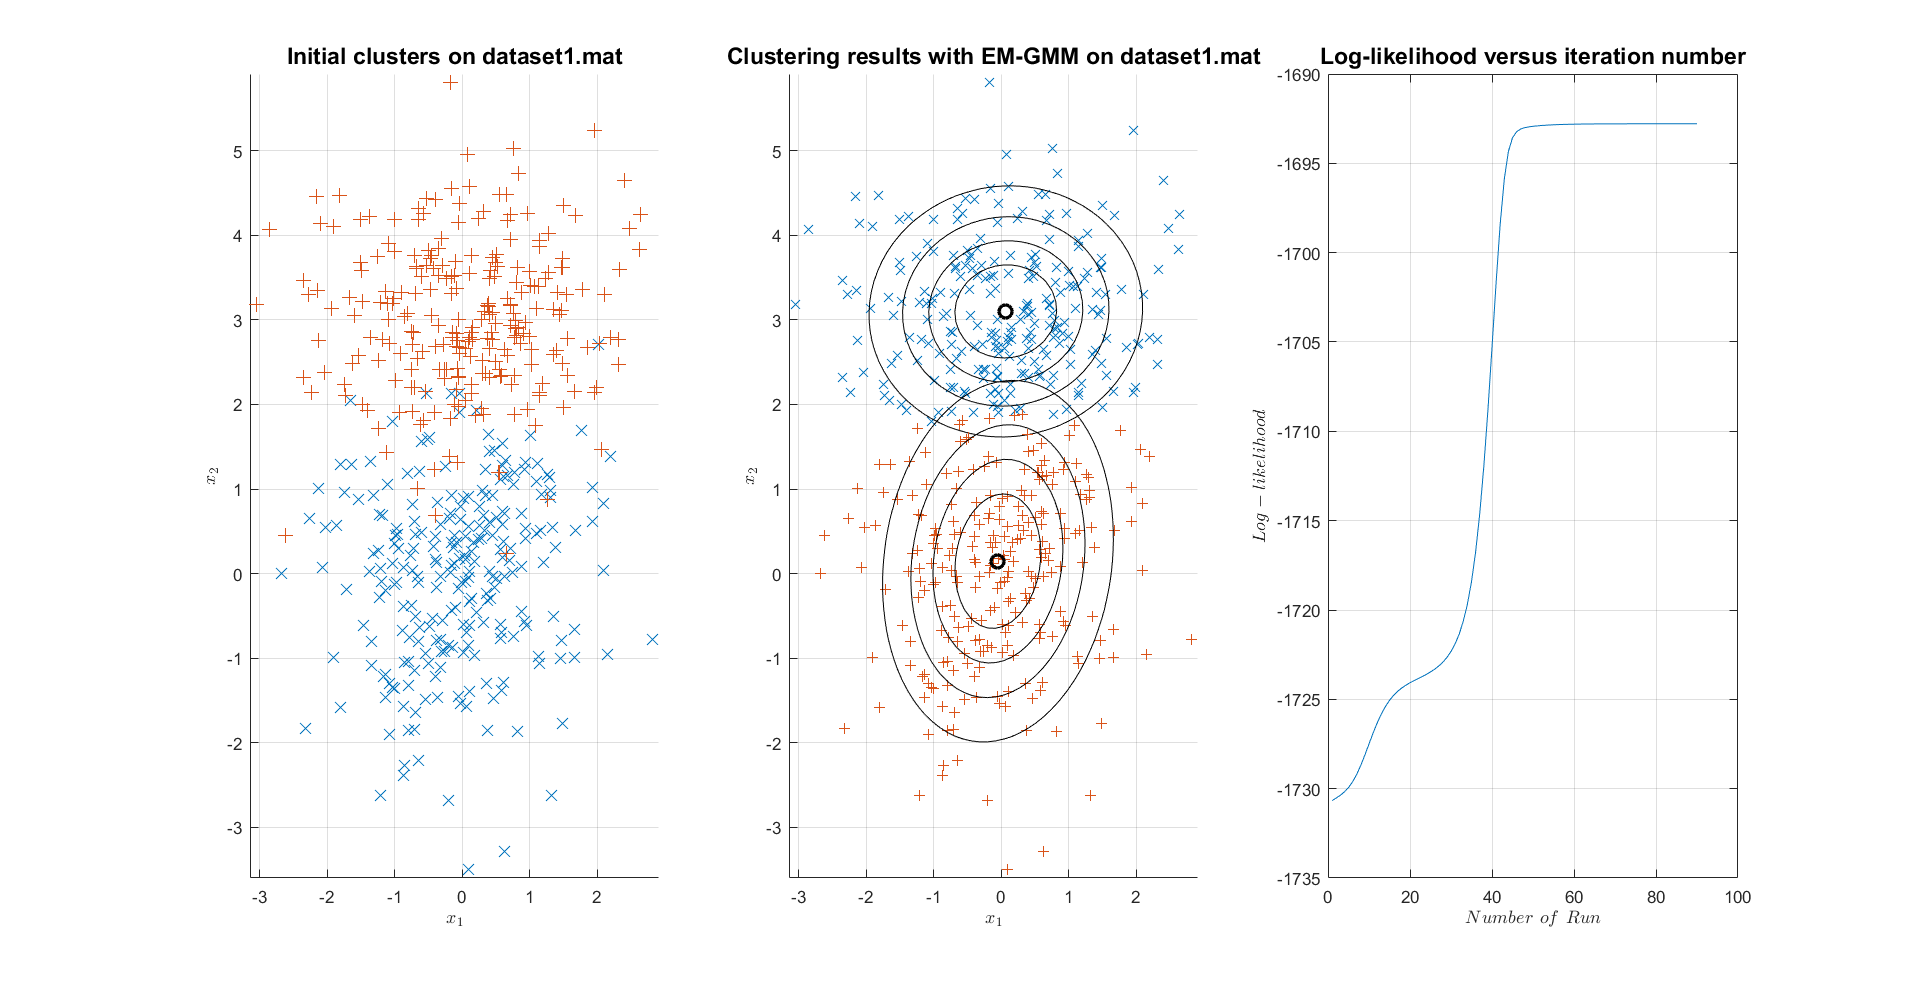
\includegraphics[width = 1\textwidth]{41b.png}
\caption{Result\ of\ clustering\ with\ EM-GMM\ on\ dataset1.mat}
\end{figure}

\begin{figure}[H]
\centering
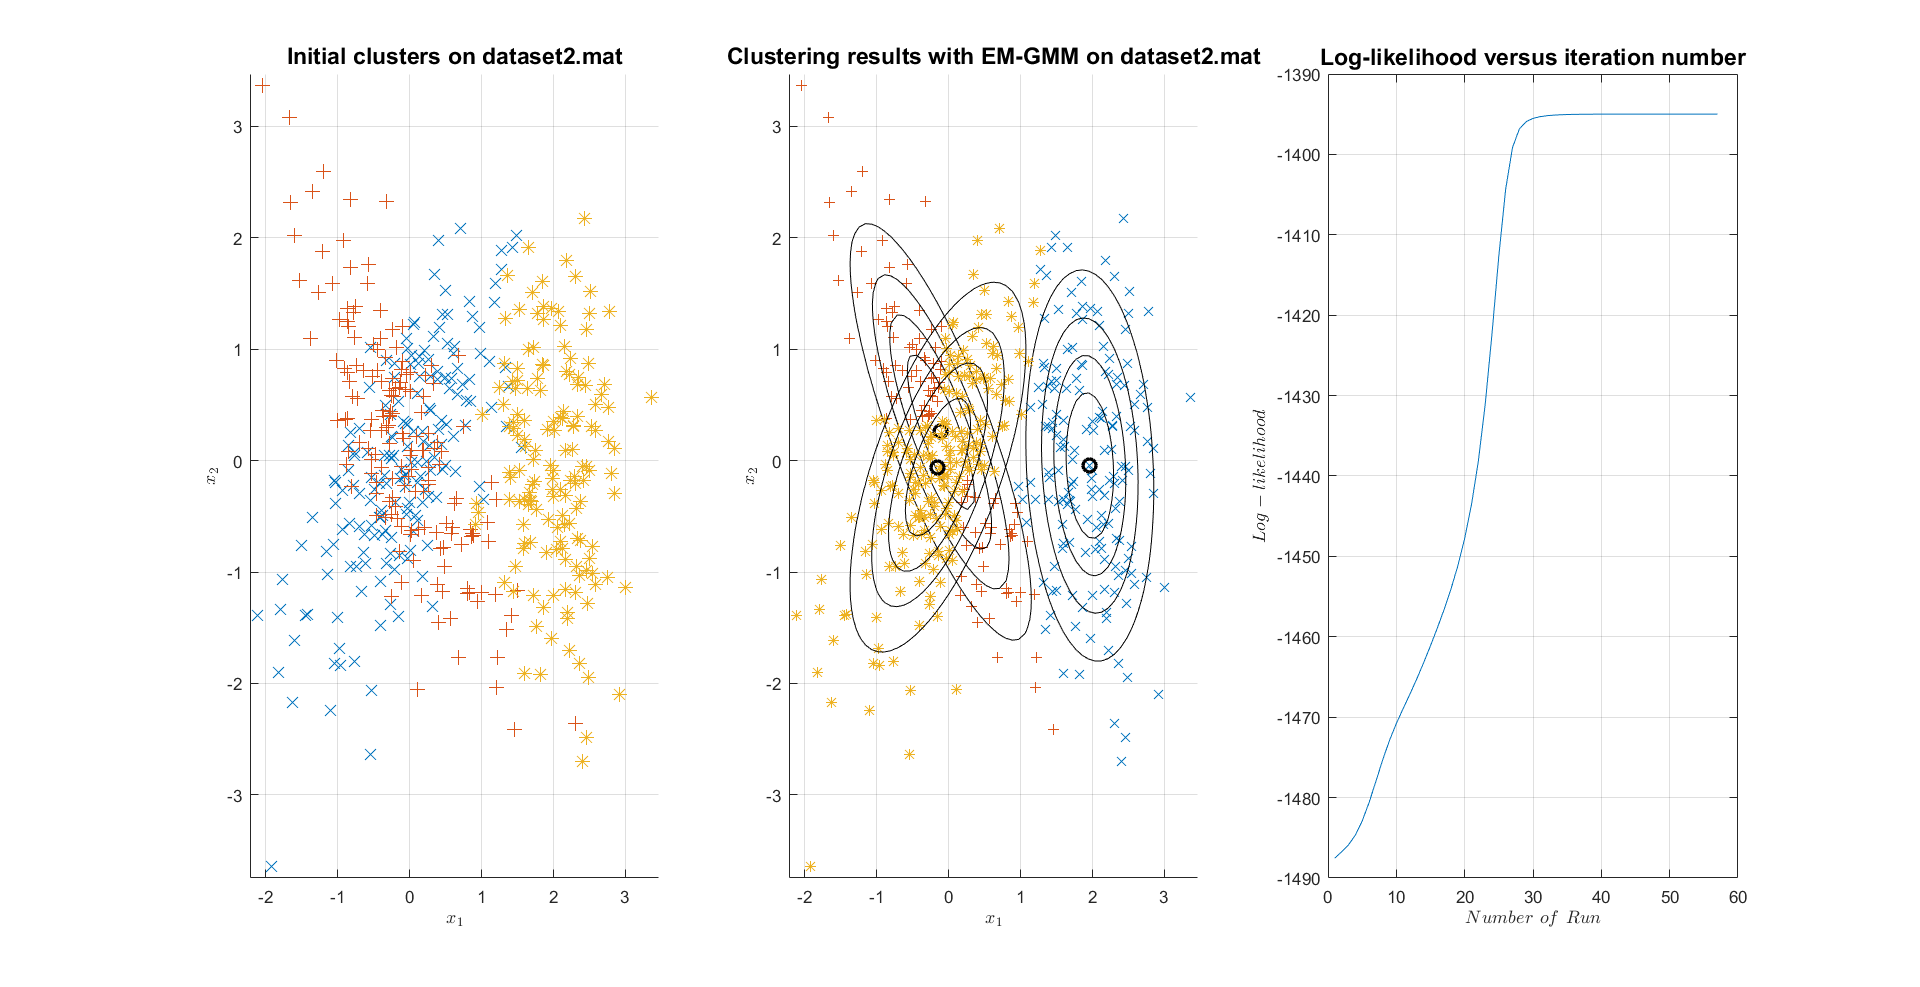
\includegraphics[width = 1\textwidth]{41c.png}
\caption{Result of clustering with EM-GMM on dataset2.mat}
\end{figure}

\vfill
\clearpage


\noindent(d) See Figure 3. Since the true clusters are radial while EM tries to fit the data points with Gaussian mixture, EM does not find the true clusters. However, EM still performs better than K-means.\\
\\
(e) See Figure 4. EM is able to capture the distribution of this non-Gaussian dataset better than K-means. 

\begin{figure}[H]
\centering
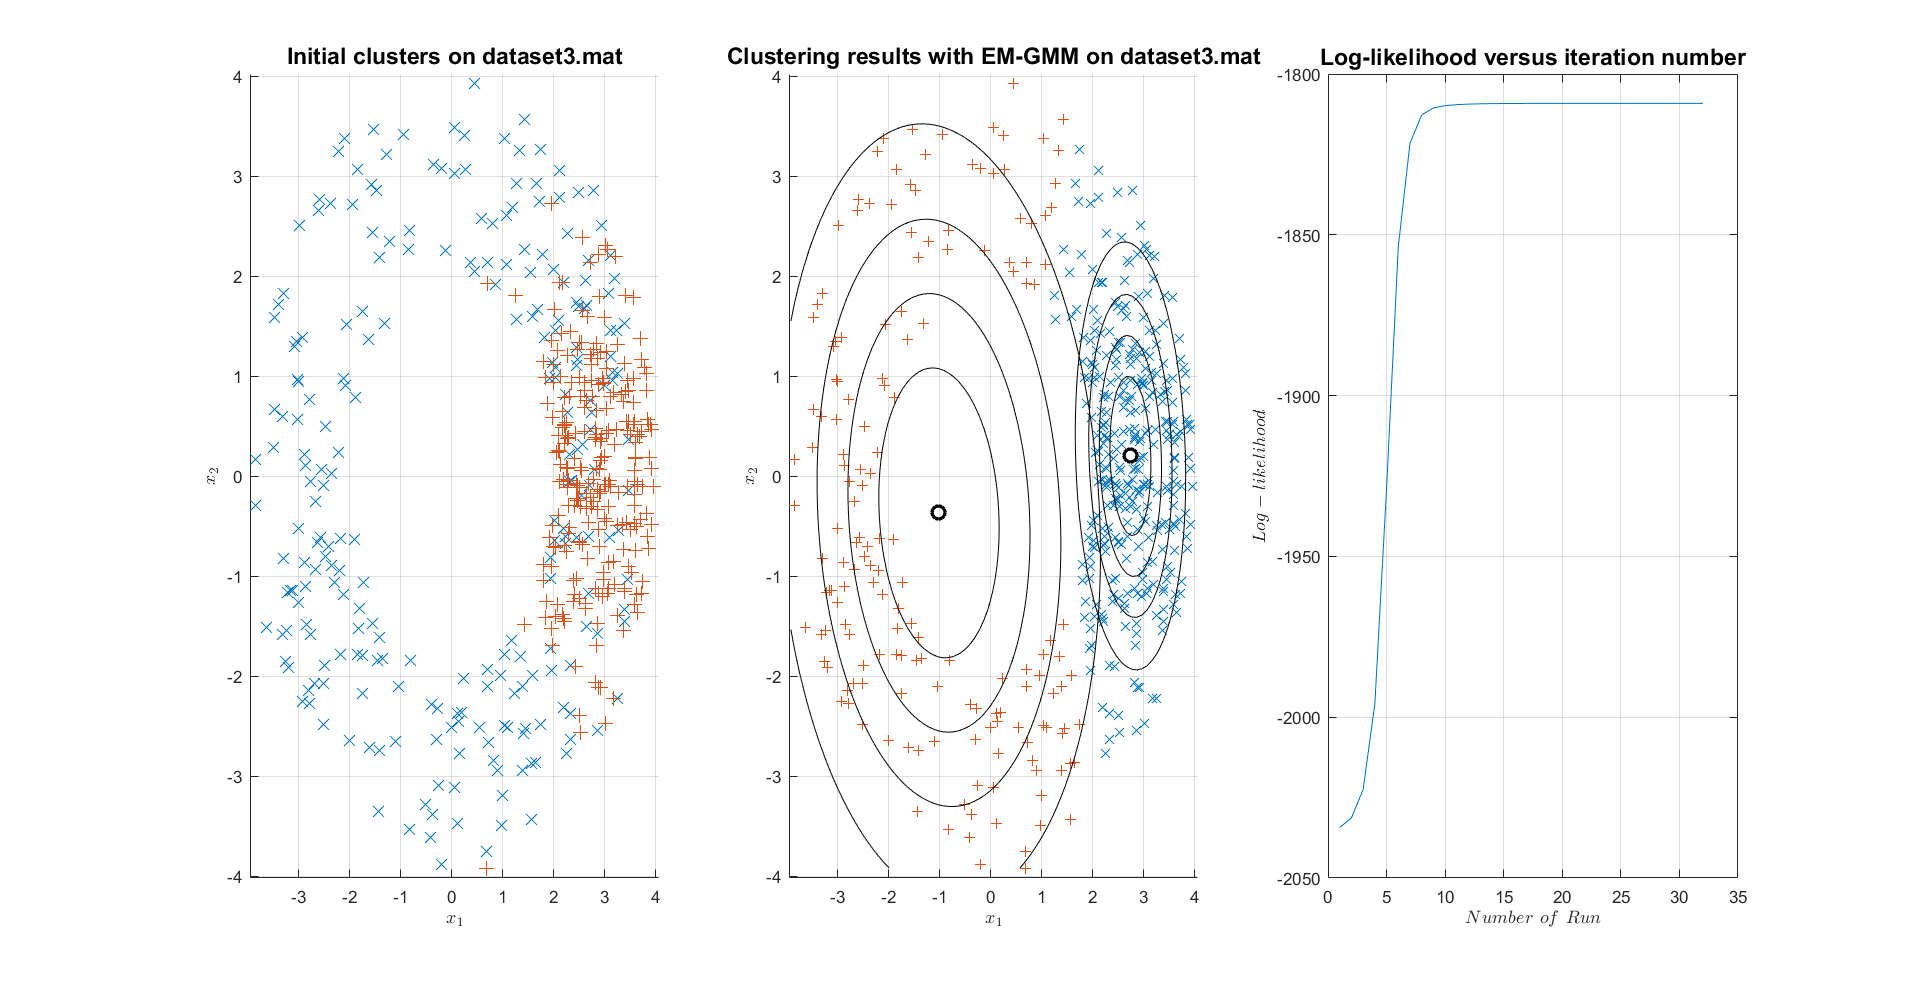
\includegraphics[width = 1\textwidth]{41d.png}
\caption{Result of clustering with EM-GMM on dataset3.mat}
\end{figure}

\begin{figure}[H]
\centering
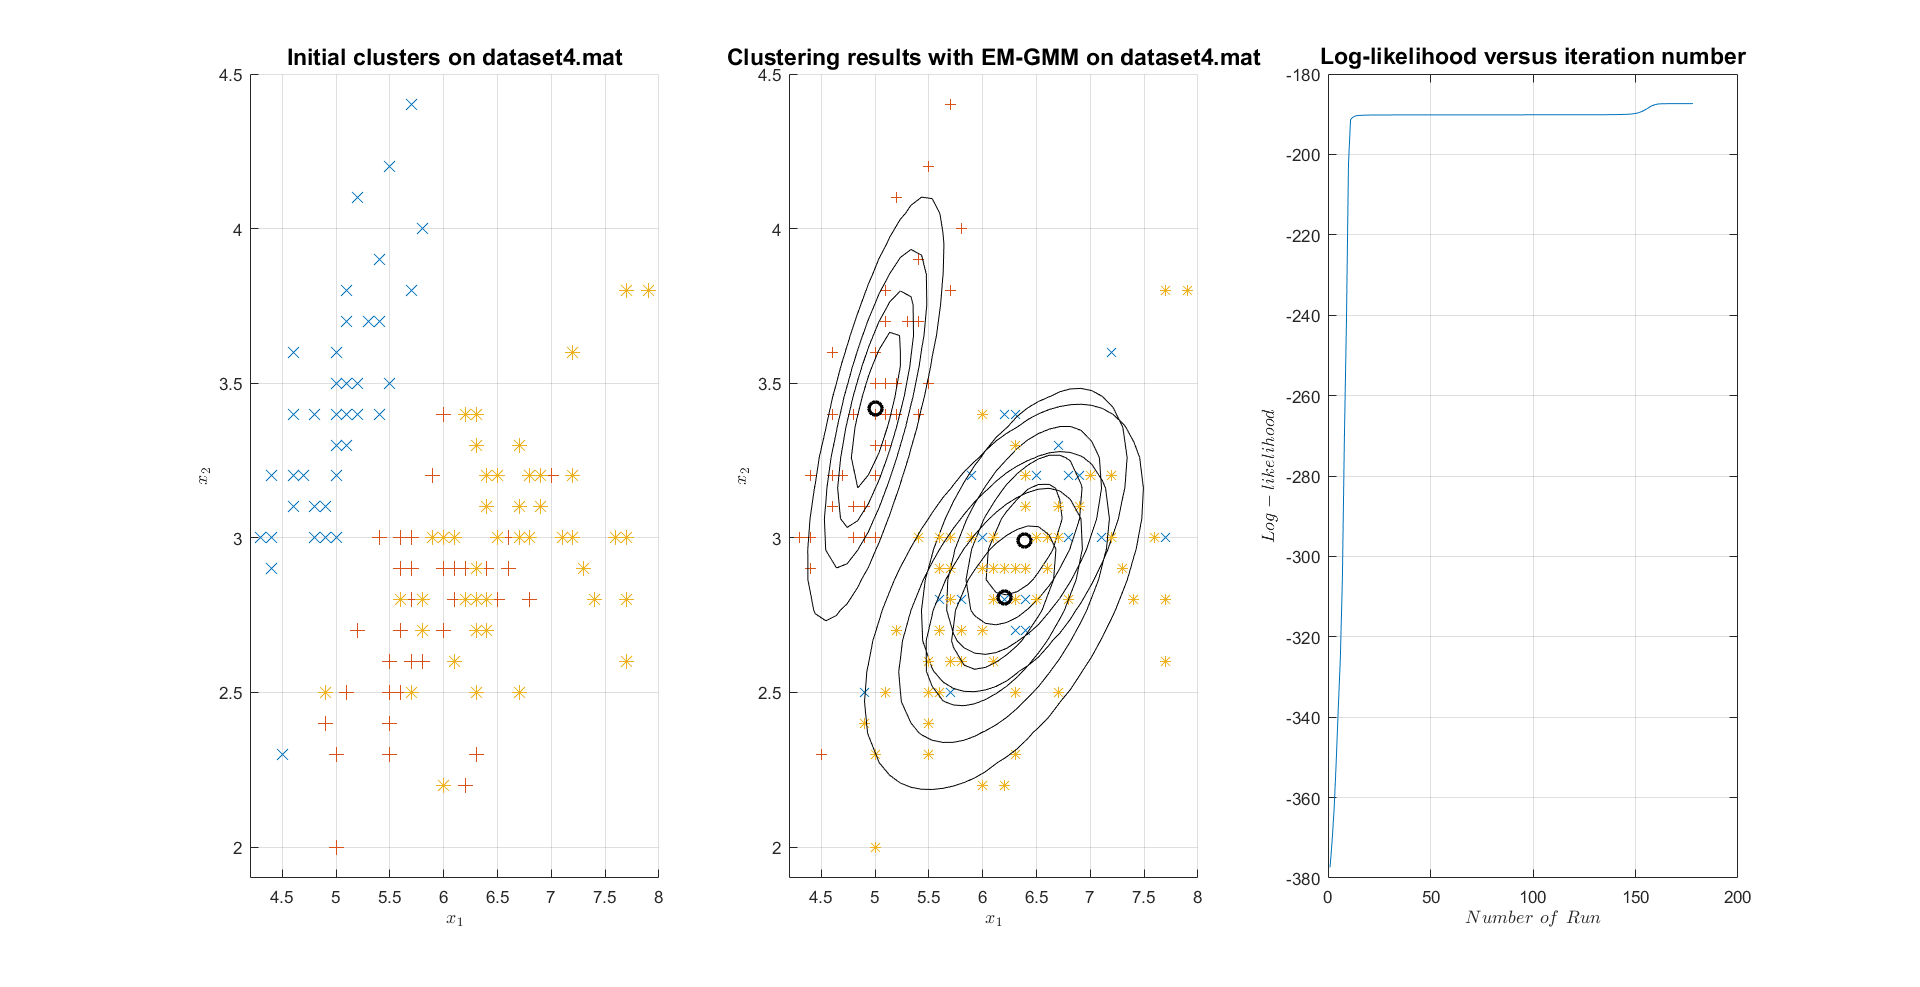
\includegraphics[width = 1\textwidth]{41e.png}
\caption{Result of clustering with EM-GMM on dataset4.mat}
\end{figure}
\vfill
\clearpage
\section{Problem 4.2}
\textbf{\begin{large}Solution:\end{large}}\\
\\
(a) See Figure 5. The maximum matches the true number of clusters.\\
\\
(b) See Figure 6. The maximum matches the true number of clusters.\\

\begin{figure}[H]
\centering
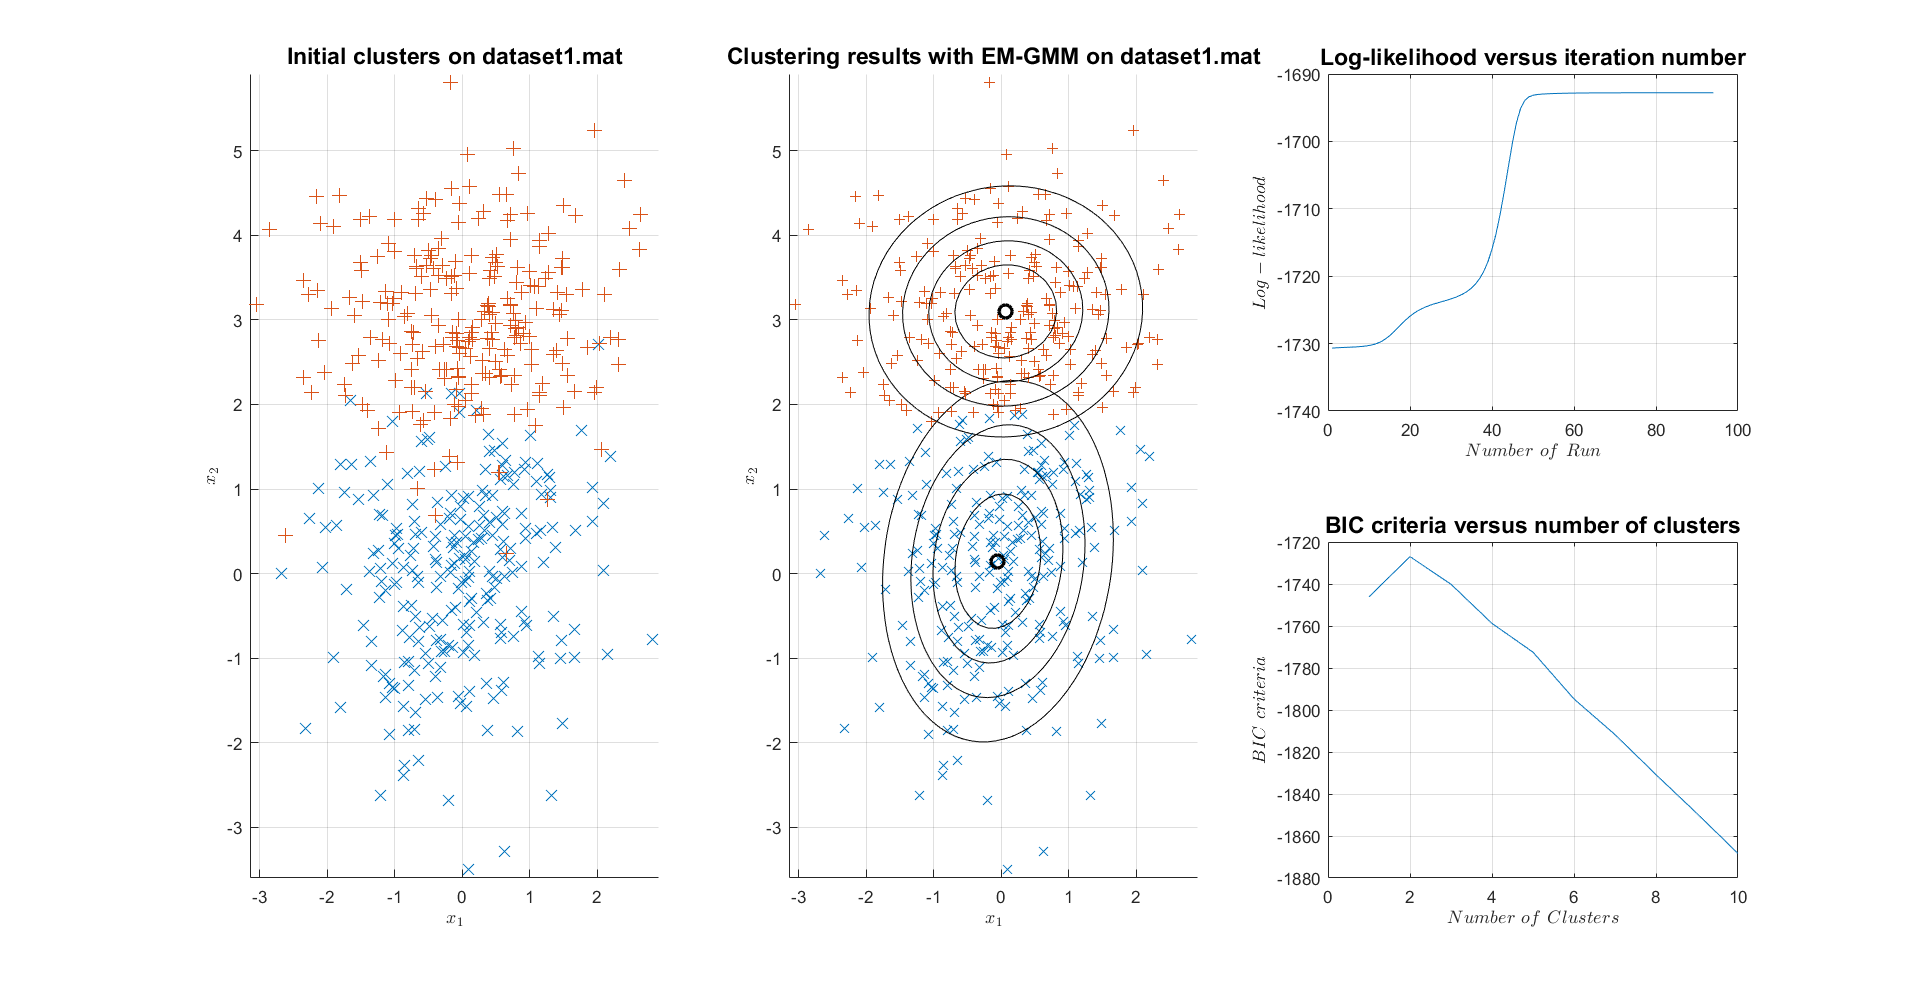
\includegraphics[width = 1\textwidth]{42a.png}
\caption{BIC result of clustering with EM-GMM on dataset1.mat}
\end{figure}

\begin{figure}[H]
\centering
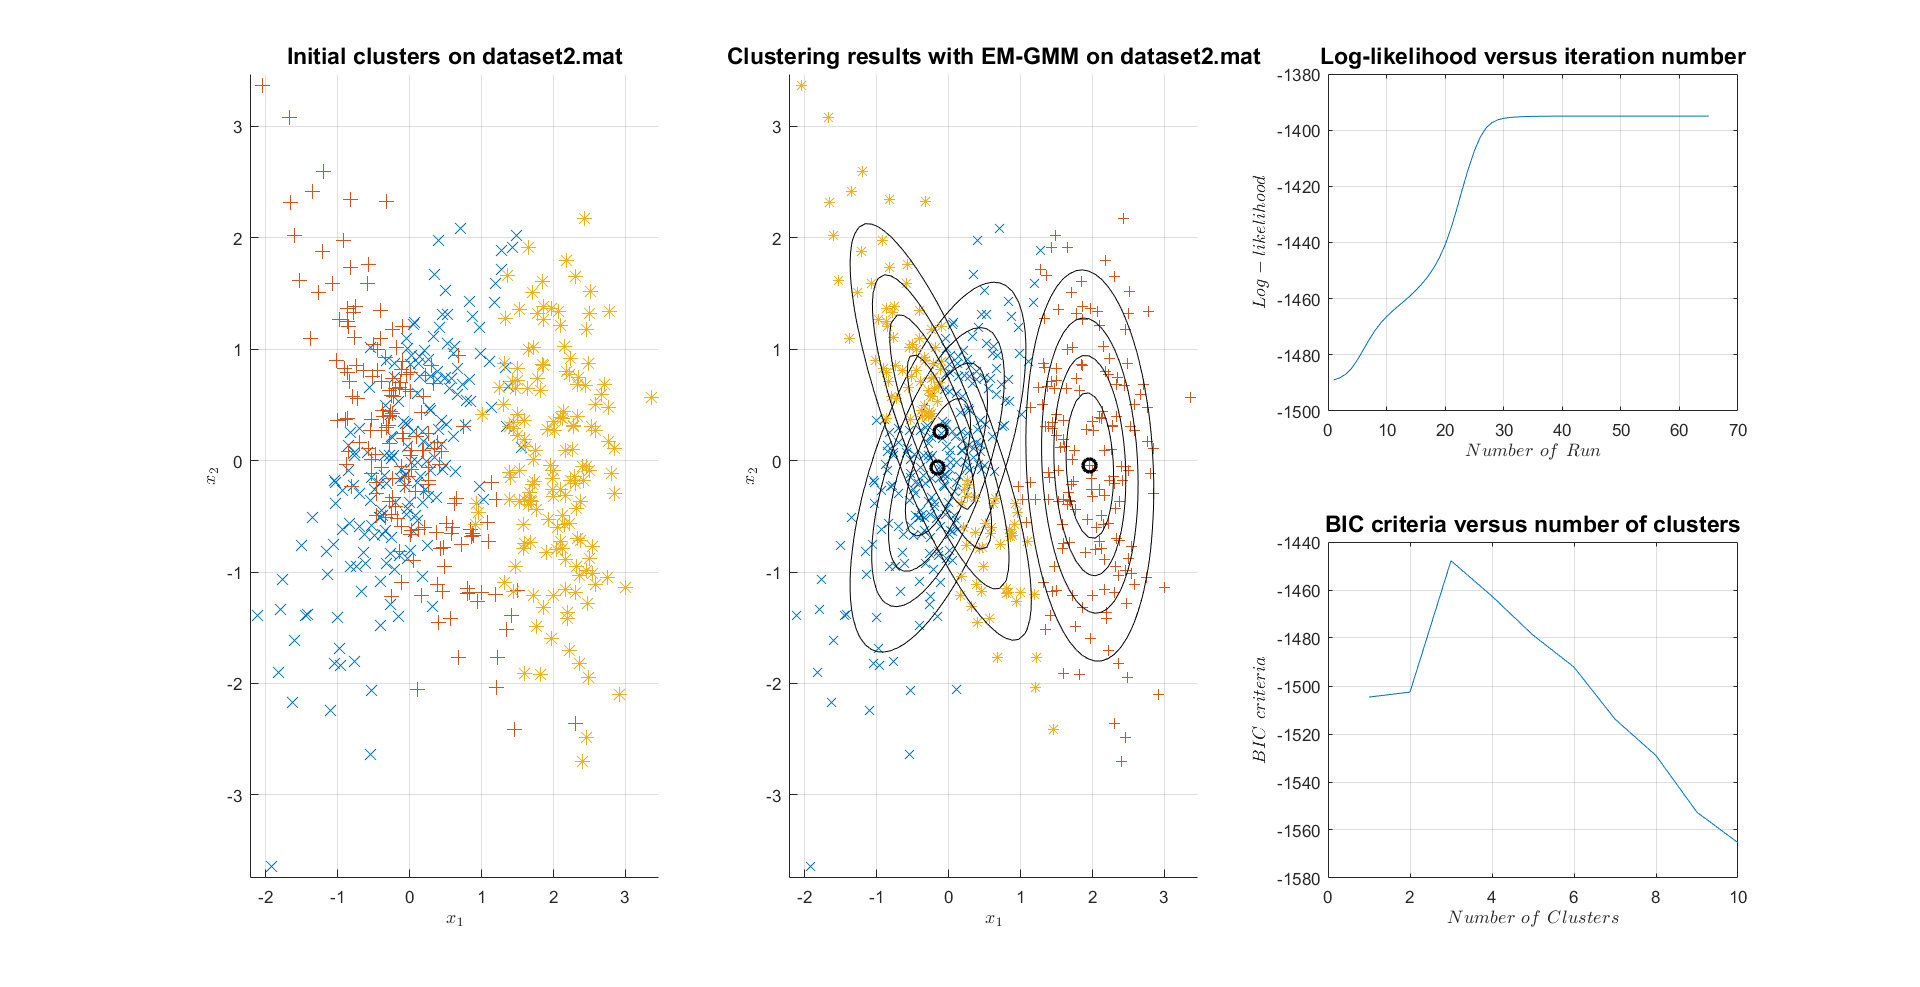
\includegraphics[width = 1\textwidth]{42b.png}
\caption{BIC result of clustering with EM-GMM on dataset2.mat}
\end{figure}
\vfill
\clearpage

\noindent(c) See Figure 7. BIC does not find the true number of clusters.\\
\\
(d) See Figure 8. The maximum matches the true number of clusters. However, there would be only two clusters in the result, which I believe depends on the initial conditions for EM algorithm.

\begin{figure}[H]
\centering
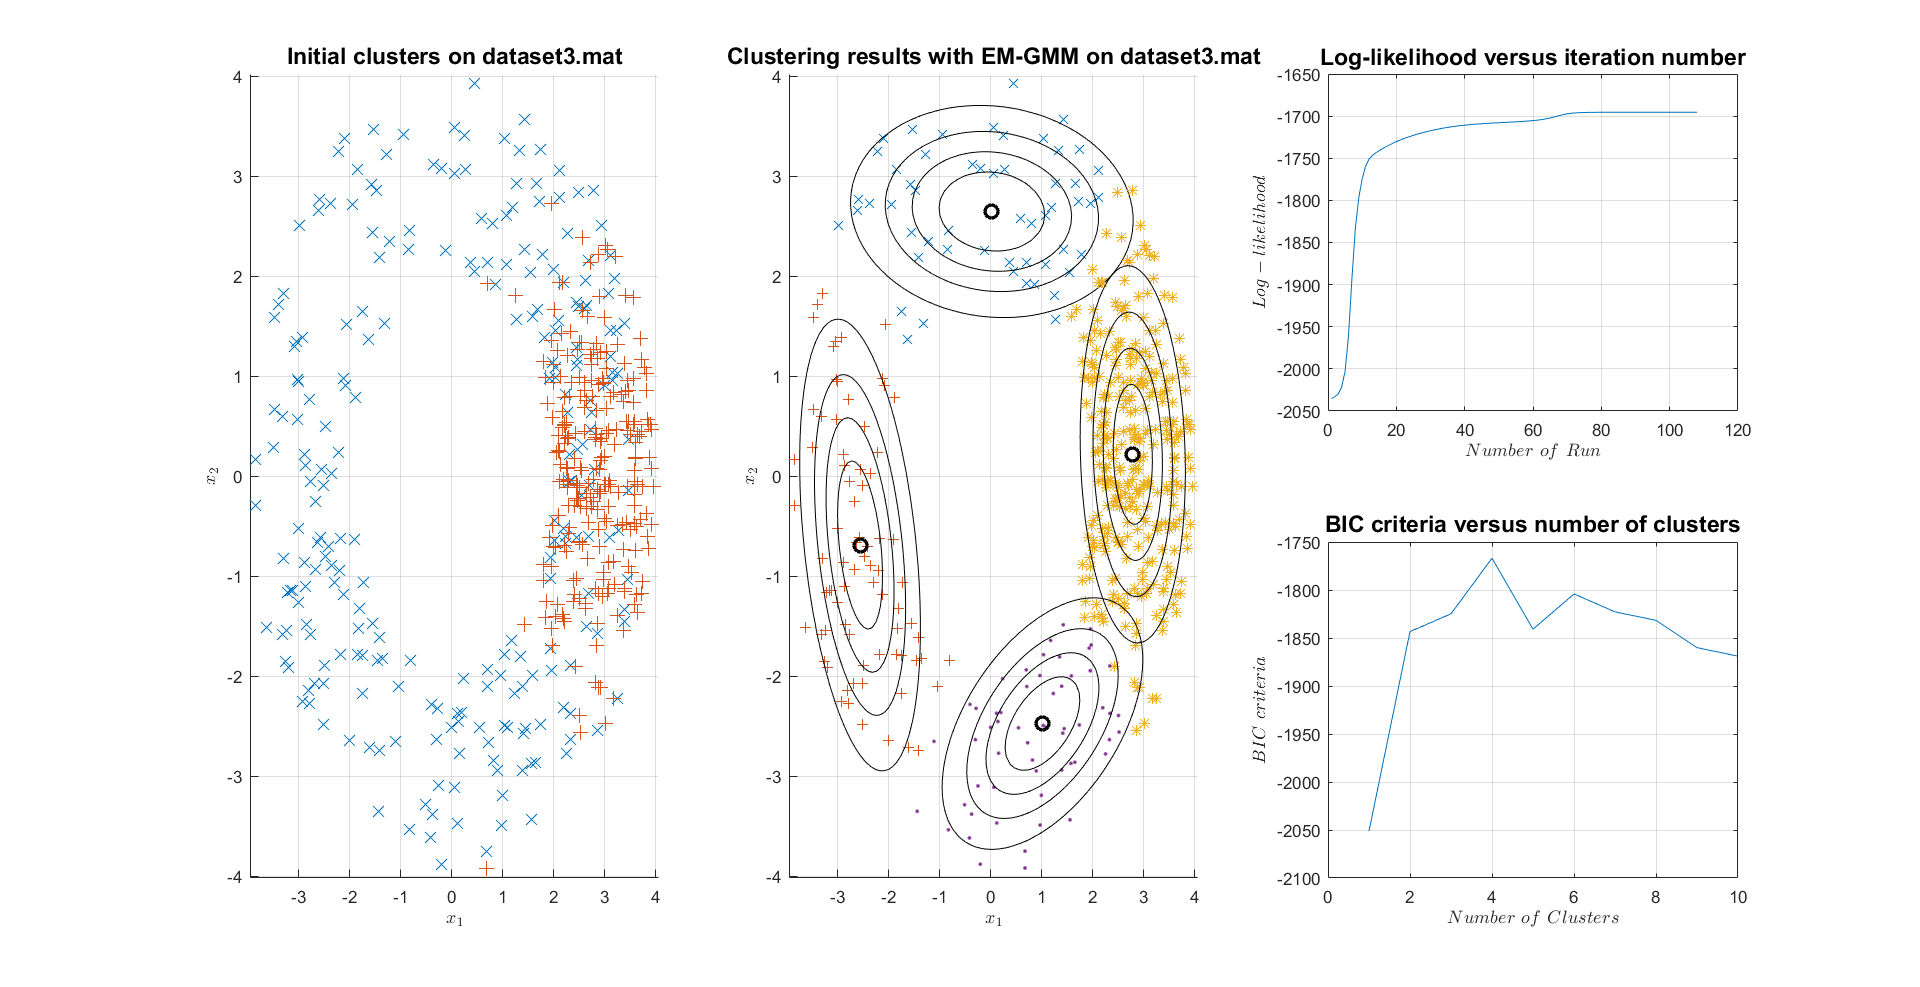
\includegraphics[width = 1\textwidth]{42c.png}
\caption{BIC result of clustering with EM-GMM on dataset3.mat}
\end{figure}

\begin{figure}[H]
\centering
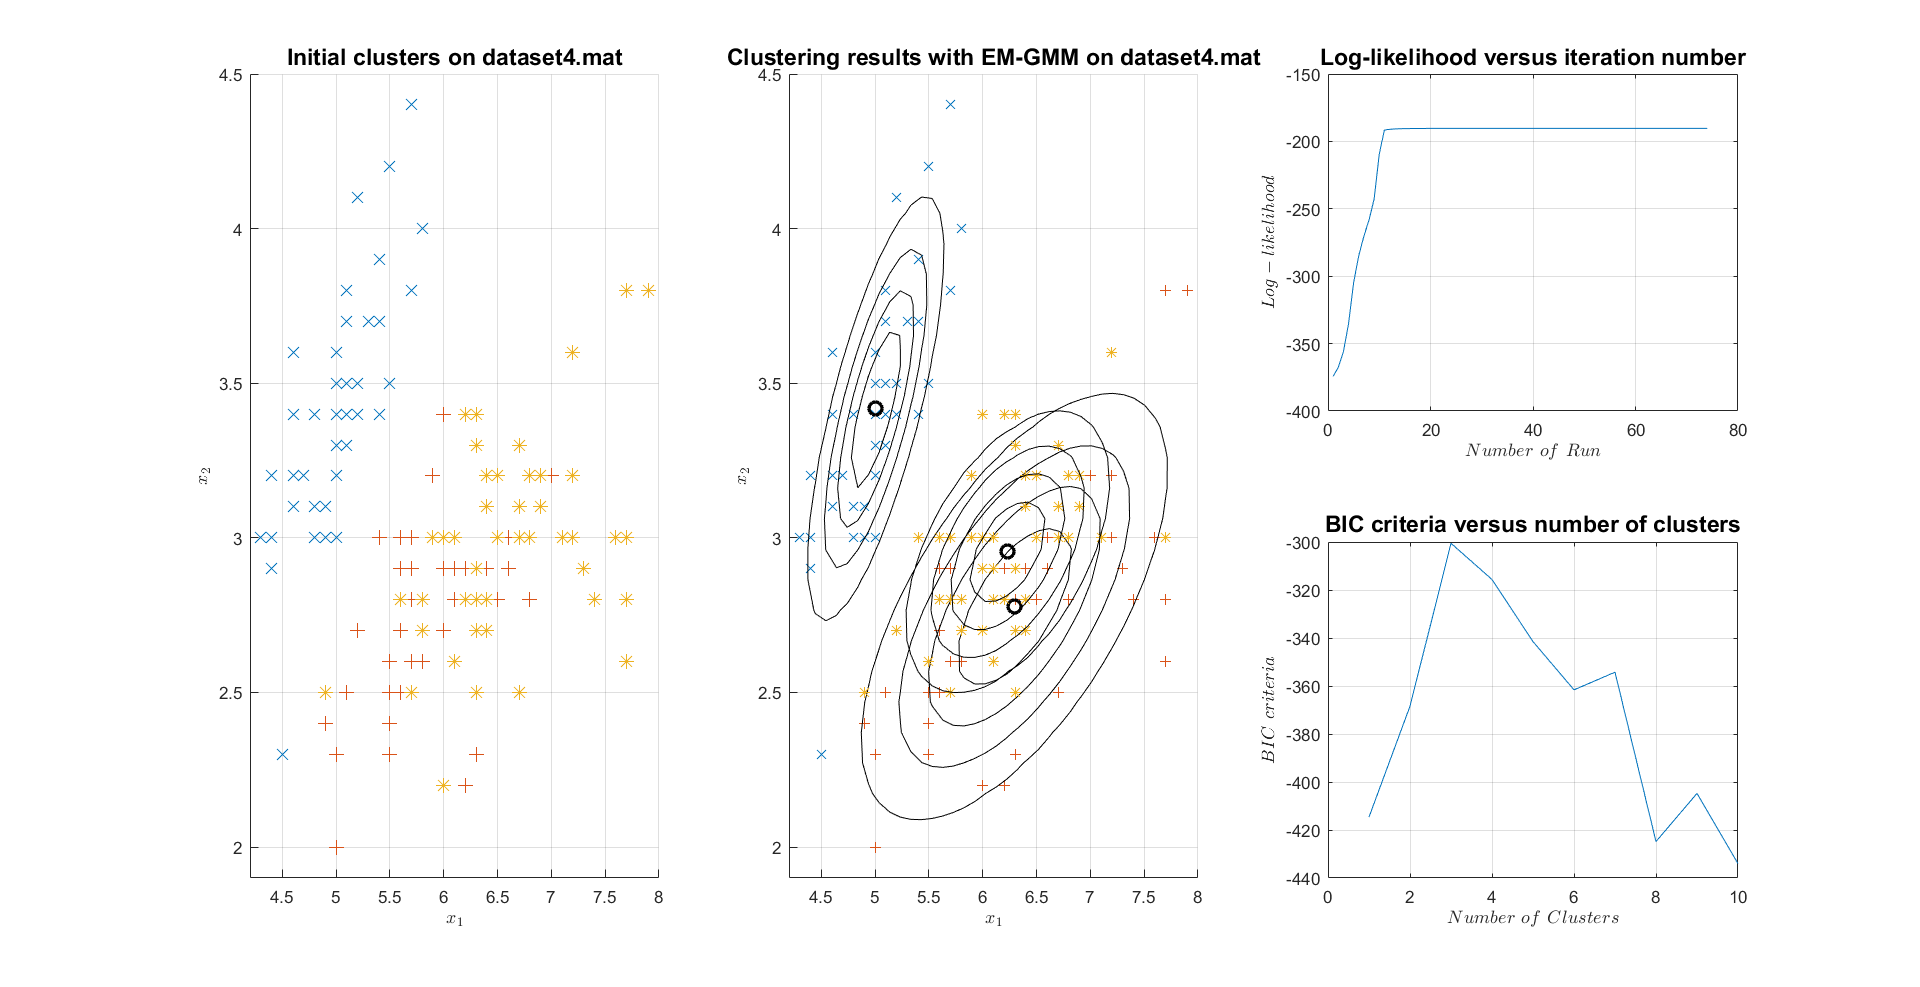
\includegraphics[width = 1\textwidth]{42d.png}
\caption{BIC result of clustering with EM-GMM on dataset4.mat}
\end{figure}
\vfill
\clearpage

\noindent(e) Both K-means and EM-GMM give the result of four clusters, but EM-GMM has a better explanation for the dataset.
\begin{figure}[H]
\centering
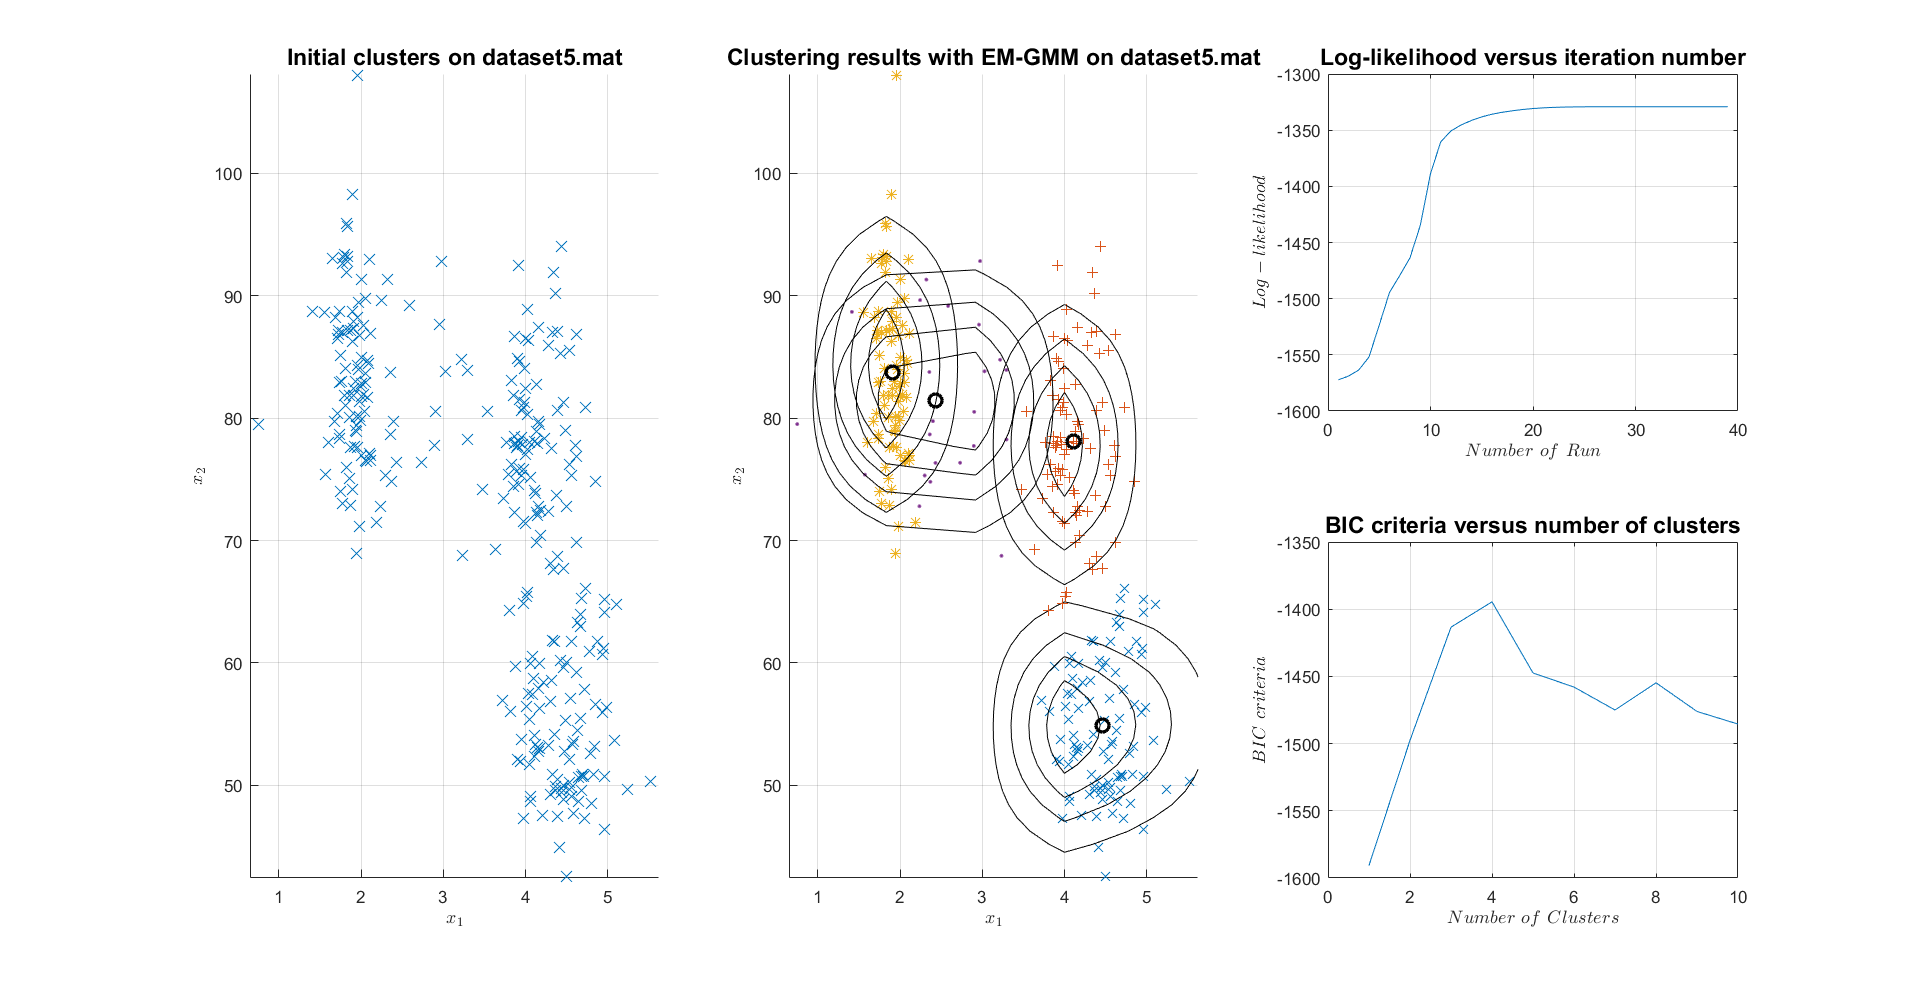
\includegraphics[width = 1\textwidth]{42e.png}
\caption{BIC result of clustering with EM-GMM on dataset5.mat}
\end{figure}


\end{document}
